
%=======================   Default Templete   ==================
\documentclass[a4paper]{article}
\usepackage{graphicx}

% file with some default definations
%%%%%%%%%%%%%%%%%%%%%%%%%%%%%%%%%%%%%%%%%
% Lachaise Assignment
% Structure Specification File
% Version 1.0 (26/6/2018)
%
% This template originates from:
% http://www.LaTeXTemplates.com
%
% Authors:
% Marion Lachaise & François Févotte
% Vel (vel@LaTeXTemplates.com)
%
% License:
% CC BY-NC-SA 3.0 (http://creativecommons.org/licenses/by-nc-sa/3.0/)
% 
%%%%%%%%%%%%%%%%%%%%%%%%%%%%%%%%%%%%%%%%%

%----------------------------------------------------------------------------------------
%	PACKAGES AND OTHER DOCUMENT CONFIGURATIONS
%----------------------------------------------------------------------------------------

\usepackage{amsmath,amsfonts,stmaryrd,amssymb} % Math packages

\usepackage{amsthm}

\usepackage{enumerate} % Custom item numbers for enumerations

\usepackage[ruled]{algorithm2e} % Algorithms

\usepackage[framemethod=tikz]{mdframed} % Allows defining custom boxed/framed environments

\usepackage{listings} % File listings, with syntax highlighting
\lstset{
	basicstyle=\ttfamily, % Typeset listings in monospace font
}

%----------------------------------------------------------------------------------------
%	DOCUMENT MARGINS
%----------------------------------------------------------------------------------------

\usepackage{geometry} % Required for adjusting page dimensions and margins

\geometry{
	paper=a4paper, % Paper size, change to letterpaper for US letter size
	top=2.5cm, % Top margin
	bottom=3cm, % Bottom margin
	left=2.5cm, % Left margin
	right=2.5cm, % Right margin
	headheight=14pt, % Header height
	footskip=1.5cm, % Space from the bottom margin to the baseline of the footer
	headsep=1.2cm, % Space from the top margin to the baseline of the header
	%showframe, % Uncomment to show how the type block is set on the page
}

%----------------------------------------------------------------------------------------
%	FONTS
%----------------------------------------------------------------------------------------

\usepackage[utf8]{inputenc} % Required for inputting international characters
\usepackage[T1]{fontenc} % Output font encoding for international characters

\usepackage{XCharter} % Use the XCharter fonts

%----------------------------------------------------------------------------------------
%	COMMAND LINE ENVIRONMENT
%----------------------------------------------------------------------------------------

% Usage:
% \begin{commandline}
%	\begin{verbatim}
%		$ ls
%		
%		Applications	Desktop	...
%	\end{verbatim}
% \end{commandline}

\mdfdefinestyle{commandline}{
	leftmargin=10pt,
	rightmargin=10pt,
	innerleftmargin=15pt,
	middlelinecolor=black!50!white,
	middlelinewidth=2pt,
	frametitlerule=false,
	backgroundcolor=black!5!white,
	frametitle={Command Line},
	frametitlefont={\normalfont\sffamily\color{white}\hspace{-1em}},
	frametitlebackgroundcolor=black!50!white,
	nobreak,
}

% Define a custom environment for command-line snapshots
\newenvironment{commandline}{
	\medskip
	\begin{mdframed}[style=commandline]
}{
	\end{mdframed}
	\medskip
}

%----------------------------------------------------------------------------------------
%	FILE CONTENTS ENVIRONMENT
%----------------------------------------------------------------------------------------

% Usage:
% \begin{file}[optional filename, defaults to "File"]
%	File contents, for example, with a listings environment
% \end{file}

\mdfdefinestyle{file}{
	innertopmargin=1.6\baselineskip,
	innerbottommargin=0.8\baselineskip,
	topline=false, bottomline=false,
	leftline=false, rightline=false,
	leftmargin=2cm,
	rightmargin=2cm,
	singleextra={%
		\draw[fill=black!10!white](P)++(0,-1.2em)rectangle(P-|O);
		\node[anchor=north west]
		at(P-|O){\ttfamily\mdfilename};
		%
		\def\l{3em}
		\draw(O-|P)++(-\l,0)--++(\l,\l)--(P)--(P-|O)--(O)--cycle;
		\draw(O-|P)++(-\l,0)--++(0,\l)--++(\l,0);
	},
	nobreak,
}

% Define a custom environment for file contents
\newenvironment{file}[1][File]{ % Set the default filename to "File"
	\medskip
	\newcommand{\mdfilename}{#1}
	\begin{mdframed}[style=file]
}{
	\end{mdframed}
	\medskip
}

%----------------------------------------------------------------------------------------
%	NUMBERED QUESTIONS ENVIRONMENT
%----------------------------------------------------------------------------------------

% Usage:
% \begin{question}[optional title]
%	Question contents
% \end{question}

\mdfdefinestyle{question}{
	innertopmargin=1.2\baselineskip,
	innerbottommargin=0.8\baselineskip,
	roundcorner=5pt,
	nobreak,
	singleextra={%
		\draw(P-|O)node[xshift=1em,anchor=west,fill=white,draw,rounded corners=5pt]{%
		Question \theQuestion\questionTitle};
	},
}

\newcounter{Question} % Stores the current question number that gets iterated with each new question

% Define a custom environment for numbered questions
\newenvironment{question}[1][\unskip]{
	\bigskip
	\stepcounter{Question}
	\newcommand{\questionTitle}{~#1}
	\begin{mdframed}[style=question]
}{
	\end{mdframed}
	\medskip
}

%----------------------------------------------------------------------------------------
%	WARNING TEXT ENVIRONMENT
%----------------------------------------------------------------------------------------

% Usage:
% \begin{warn}[optional title, defaults to "Warning:"]
%	Contents
% \end{warn}

\mdfdefinestyle{warning}{
	topline=false, bottomline=false,
	leftline=false, rightline=false,
	nobreak,
	singleextra={%
		\draw(P-|O)++(-0.5em,0)node(tmp1){};
		\draw(P-|O)++(0.5em,0)node(tmp2){};
		\fill[black,rotate around={45:(P-|O)}](tmp1)rectangle(tmp2);
		\node at(P-|O){\color{white}\scriptsize\bf !};
		\draw[very thick](P-|O)++(0,-1em)--(O);%--(O-|P);
	}
}

% Define a custom environment for warning text
\newenvironment{warn}[1][Warning:]{ % Set the default warning to "Warning:"
	\medskip
	\begin{mdframed}[style=warning]
		\noindent{\textbf{#1}}
}{
	\end{mdframed}
}

%----------------------------------------------------------------------------------------
%	INFORMATION ENVIRONMENT
%----------------------------------------------------------------------------------------

% Usage:
% \begin{info}[optional title, defaults to "Info:"]
% 	contents
% 	\end{info}

\mdfdefinestyle{info}{%
	topline=false, bottomline=false,
	leftline=false, rightline=false,
	nobreak,
	singleextra={%
		\fill[black](P-|O)circle[radius=0.4em];
		\node at(P-|O){\color{white}\scriptsize\bf i};
		\draw[very thick](P-|O)++(0,-0.8em)--(O);%--(O-|P);
	}
}

% Define a custom environment for information
\newenvironment{info}[1][Info:]{ % Set the default title to "Info:"
	\medskip
	\begin{mdframed}[style=info]
		\noindent{\textbf{#1}}
}{
	\end{mdframed}
}

\usepackage{listings}
\lstset{language=Python, basicstyle=\normalsize\sffamily\linespread{0.8}, numbers=left, numberstyle=\small, stepnumber=1, numbersep=5pt}
\usepackage{fancyhdr}
\usepackage{pdfpages} 
\setlength{\parindent}{0pt}

\pagestyle{fancy}
\fancyhf{}
\lhead{\textbf{\NAME\ (\ANDREWID)}}
\chead{\textbf{UGP Report}}
\rhead{\COURSE}


%==================Header details======================
\newcommand\NAME{Raghukul Raman Sudhanshu Jaiswal Chaman Agarwal}
\newcommand\ANDREWID{}
\newcommand\HWNUM{4}
\newcommand\COURSE{CS395}
%======================================================

% available formatted sections:
% - COMMAND LINE ENVIRONMENT: \begin{commandline} \end{commandline}
% - FILE CONTENTS ENVIRONMENT: \begin{file}[optional filename, defaults to "File"]
% - NUMBERED QUESTIONS ENVIRONMENT: \begin{question}[optional title]
% - WARNING TEXT ENVIRONMENT(can also be used for note): \begin{warn}[optional title, defaults to "Warning:"]
% - INFORMATION ENVIRONMENT(can be used to mention given details): \begin{info}[optional title, defaults to "Info:"]

%===============================================================
\begin{document}
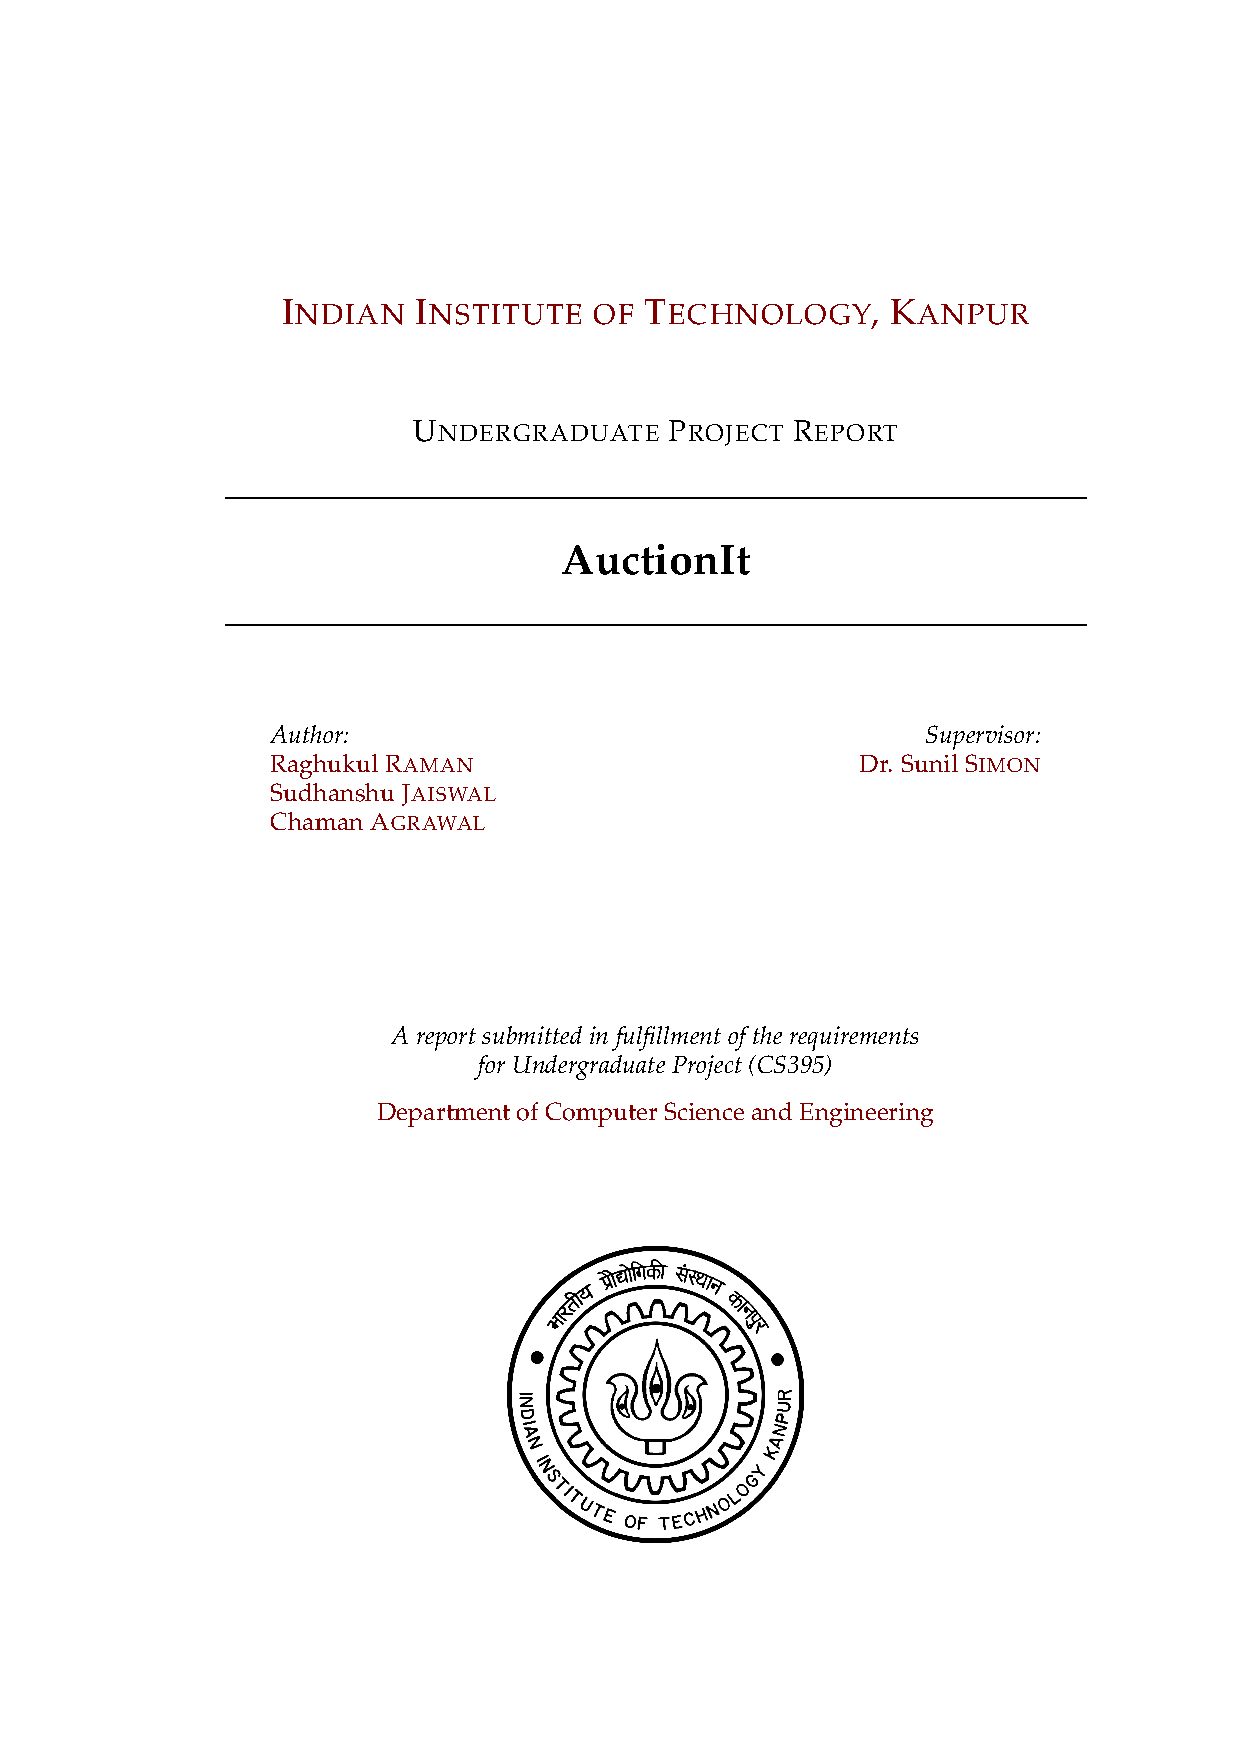
\includepdf[page={1}]{first_page.pdf}
\section*{Abstract}
An auction is a process of buying and selling goods or services by offering them up for bid, 
taking bids, and then selling the item to the highest bidder. 
So why are auctions important? In nutshell, it is important because certain goods might have some value to the seller,
and therefore the seller might have some reserved price below which the she would not be willing to sell.
If left to the market, the price might fall below that price.
Also, there do exist willing buyers who are ready to pay the higher value.
Moreover it has become a method of determining prices of goods. \\
Some salient features of using an auction are:
\begin{itemize}
	\item Speedy Process, Quick Turnaround.
	\item Competitive Bidding.
	\item Auctions Work Well in Both Good and Bad Economic Times.
	\item No Negotiations.
	\item can get good idea of price.
	\item You Know Exactly When Your Property or Goods Will Be Sold.
	\item and may more...
\end{itemize}
Auctions have become an integral part of today's world, they are used extensively in almost every field. Some widely used auctions are spectrum auction, treasury auction, auction for advertisement, auctions for players such as in IPL or EPL leagues.\\ \\
Considering the need for auctions, we hereby present a software, which is generic enough to conduct several different auctions called \textbf{Auctionit}.
\\

\section*{Introduction}
AuctionIt allows auction designers to create and host auctions, users can place bids on items in the auction and can see the results and price they have to pay at the end of the auction process. Auction Designers can modify and create new fields which allow them to get more data from the bidders that is relevant to the auction being held. They can also choose from pre-defined auction templates to quickly set up some of the more common auctions. They can also define their custom allocation rules and pricing rules. This allows to set up complicated rules for pricing and allocation and thus provides more freedom to the designer to create a wide variety of auctions. 
The software, categorizes auction designers and bidders as different types of users. These accounts are password protected to prevent misuse and to ensure the auction is not compromised while it runs.

Before we started designing AuctionIt, we studied about auctions. We read papers/lectures to understand the reasons why first price and second price auctions are so popular and widely used. We also read and learnt about the auction process for large scale real life auctions take place like treasury auctions or spectrum auctions. We read about auctions with multiple objects and how these large scale auctions deal with having multiple objects which may be similar and how they setup rules to prevent allocating a majority of a commodity to a particular set of bidders.
\section*{Theory Review}


We read a paper on the problem of reallocation of the radio frequencies given to television stations, so as to clear spectrum for wireless internet access. The major challenges that are faced to conduct such an auction are:\\
1) The channels to and their geographical locations need to be continuous for wireless so each owner becomes essential and can demand a higher price.\\
2) Spectrum interference is required to be tackled while maintaining price clearing and continuous reallocation.

To overcome these challenges an Incentive auction is conducted. An incentive auction consists of two separate auctions - a backward auction to determine the price at which broadcasters will sell their spectrum usage rights and a forward auction to identify the prices companies will pay for wireless allocation. Both forward and backward auctions are VCG auctions and belongs to a class of deferred acceptance algorithm, forward auction's bidding increases with rounds while the back auction is a decreasing clock auction.
\\\\
We start by introducing First Price and Second Price auctions, which are the two most common types of auctions held around the world. 
\\\\
\textbf{First Price Auctions :} In a first price auction, all the bidders submit their sealed bids and then the highest bidder wins the auction while paying the price he bid. Though very commonly used, the first price auction is not incentive compatible. This means that the bidders will not achieve the best outcome by bidding an amount equal to his true valuation of the object(s). Since the profit for the bidder is Value - Bid, it makes sense to bid lower than his own valuation of the object. 
\\\\
\textbf{Incentive Compatibility :} An auction mechanism is said to be Incentive Compatible if every participant can achieve the best outcome to himself just by bidding at his own true valuation. 
\\\\
\textbf{Dominant-Strategy-Incentive-Compatible (DSIC) :} This a strong form of Incentive Compatibility where a bidder fares the best by being truthful regardless of what the other bidders act like. 
\\\\
\textbf{Second Price Auctions :} In a second price auction, all the bidders submit their sealed bids and the highest bidder wins the auction while paying the price of the \textbf{second highest} bidder. Unlike the first price auction mechanism, the second price auction is Incentive Compatible. Infact, it is DSIC, which means it is in the best interest of the bidder to submit his true valuation as the bid itself. 
\subsection*{Treasury Securities auctions}

\paragraph{Treasury securities :}Treasury securities or Treasuries are bonds issued by the government to meet their financial debts. Based on the period of maturity they are categorized into different types that are Treasury bills, notes, bonds, and Treasury inflation-protected securities.
\\\\
Most of the treasury auctions come in one of the two categories of auctions: Discriminatory Price auction and Uniform Price auction.
\\\\
\textbf{Discriminatory-Price auction :} In Discriminatory Price auction, allocation rule is that the bidder with the highest bid wins and the winner pays his own bid, so this reduces to the first-price auction in case of a single object auction.
\\\\
\textbf{Uniform-Price auction :} In this, the allocation rule is same as Discriminatory Price auction, that is the winner with the highest bid wins but in this case, all winners pay an averaged uniform price and this cuts to the second-price auction in single item auction.
\\\\
Treasury auctions are different from other auctions as the values of these securities in the secondary market in known before the auction and are independent of the private valuation of the bidders. These type of auctions are called common value auctions. This difference in valuation results in a phenomenon called 'winner's curse' which is a significant factor in choosing between the above two pricing rules for revenue maximization proper of the above two price rules.
\\\\
\textbf{Winner's Curse :} In a common value auction the real value of the item is the same for all the bidders, but they bid differently according to their estimate of the secondary market value. If we take the average of all the bids as an estimate of the actual secondary market value, then the highest bidder incurs the highest loss by winning the item at such a high price.
\\\\
From the definition of the winner's curse, it can be observed that the winning bidder will suffer more loss in the case of discriminatory price auction than uniform price auction. This causes the bidders to bid less than there valuation and results in lower revenue.
\\\\
Hence the Uniform-price method is more efficient than the Discriminatory-price method regarding revenue generation, but several surveys reveal that Discriminatory-price method dominates in Treasury auctions in most parts of the world and so this is an example of a situation where theory and practice do not agree woth each other.

\subsection*{US Radio spectrum reallocation}

The following is a study of the process used for the US radio spectrum reallocation given to television stations and clear spectrum for wireless internet service providers.
\\\\
The spectrum reallocation process is a complex one and needs to handle multiple challenges like how many television channels to reallocate, which channels to reassign, how to determine compensation for reassignment, how to distribute the cleared spectrum to the wireless companies etc. One of the major problems is that the channels cleared and their geographical location needs to be continuous for the wireless broadband purpose. The continuity requirement of channels and their geographic location makes even small owners important, and thus each broadcaster can ask for a higher price, exploiting his/her importance for the whole project. Other than these multiple problems the computational issues are also a concern. It is computationally expensive to check for interference constraints, and these checks are required for each reassignment.
\\\\
The auction to reassign spectrum, which came to be known as the 'incentive auction', involved bidding by both buyers and sellers.
\\\\
\textbf{Incentive auction:} This consists of two separate auctions - a backward auction to determine the price at which broadcasters will sell their spectrum usage rights and a forward auction to identify the prices companies will pay for wireless allocation. Both forward and backward auctions are VCG auctions and belong to a class of deferred acceptance algorithm, forward auction's bidding increases with rounds while the back auction is a decreasing clock auction.

\subsubsection*{VCG for the incentive auction}

In a VCG auction if the price of one player is a nondecreasing function of the bid by another player then they are called substitutes on the other hand if the price is a nonincreasing function of the other player's bid then they are called complements. Aggressive bidding by substitutes is desired as it will reduce the price of the radio spectrum.
\\\\
If one does not have to care about the cost of reallocation, then VCG auction will be an optimal choice that will promote truthful bidding and maximizes revenue. Each bid independently of other bidders and since each player bids regardless of the others the dominant strategy will be to bidders to bid their valuations. In the same way, the radio station will sell his license only when the price is strictly higher than his estimate.
\\\\
In the real incentive auction, a large number of stations are needed to clear even little spectrum for nationwide usage so the cost of reallocation cannot be ignored. This problem is solved by the changed property rights of television stations. The station only has right for interference-free coverage in some channel. As a result, the price of stations reduced since if the price is too high, it can be reassigned to a different channel. This promotes competition among the channels and makes them substitutes.
\\\\
So an unmodified VCG auction is not suitable for incentive auction because:

\begin{description}

\item[$\bullet$] It generally runs a budget deficit.
\item[$\bullet$] It is computationally hard to solve the value maximization reallocation problem with millions of interference constraints subjected.
\item[$\bullet$] The success of auction depends on the participation of small broadcasters. They may find the auction mechanism complex and decline to participate at all.

\end{description}

\subsubsection*{Modified VCG for the incentive auction}

A Heuristic Clock Auction for incentive auction achieves high efficiency and more straightforward computation process and still strategy-proof. The design involves bidding in two auctions: a reversed auction for government to buy broadcasting rights from radio stations and a forward auction to sell the cleared spectrum to the wireless broadcasters. In each of the auctions, the auctioneer asks players to submit offers and then iteratively rejects them one by one. The auctioneer may allow the rejected player to offer again. At the end of the auction, all the offers that are not dismissed are accepted.
\\\\
The reverse is a decreasing clock auction in which the auctioneer quotes a decreasing sequence of prices, and the players indicate if they are willing to sell at that price or not. If not they leave the auction irreversibly. When the auction ends, all the remaining players sell their rights at the last quoted price. A similar approach is used in the forward auction to sell the rights to the wireless broadcasters.


\section*{Design Details}
For the design, we can seperate AuctionIt into two major sections -  the database and the main program/front end. The database consists of the following set of tables : - \\
\begin{enumerate}
    \item \textbf{User} Table\\
     - The user table stores information about the user and also his login credentials such as username and password details.
    \item \textbf{Designer} Table\\
    - The designer table stores the login credentials for the auction designers, it also stores a list of past auctions created by the designer with auction-id and revenue generated by the auction. If the designer has created custom allocation and pricing rules then we store their ids (from Table 7 and Table 8) for easy access while creating later auctions.
    \item \textbf{Default Auction} Table
    \item \textbf{Live Auction} Table
    \item \textbf{Bid} Table
    \item \textbf{Ranking} Table
    \item \textbf{Allocation Rules} Table
    \item \textbf{Pricing Rules} Table
\end{enumerate}
\section*{Further improvements}

\section*{References}
\end{document}

